\documentclass[10pt]{report}

\usepackage{geometry}
\geometry{
	letterpaper,
	hmargin=1in,
	vmargin=1in,
	footskip=0.25in
}

\usepackage{enumerate} % for enumerate counter
\usepackage{subcaption} % for subfigures
\usepackage{amsthm} % for QED
\usepackage{mathtools} % for delimiter

\usepackage{listings} % for code
\lstset{ 
	language=R,
	basicstyle=\footnotesize\ttfamily,
	numbers=none,
	stepnumber=1,
	numbersep=8pt,
	showspaces=false,
	showstringspaces=false,
	showtabs=false,
	frame=single,
	tabsize=2,
	captionpos=t,
	breaklines=true,
	breakatwhitespace=false
} 

\usepackage{float} % for figure [H]
\usepackage{booktabs} % for tabular
\usepackage{caption} % for \caption*
\usepackage[export]{adjustbox} % for valign=t
\usepackage{array} % for column type m
\usepackage{verbatim}
\usepackage{graphicx}
%\graphicspath{ {imgs/} }

\usepackage{fancyhdr}
\pagestyle{fancy}
\fancyhead[L]{\hwAuther}
\fancyhead[C]{\courseNo}
\fancyhead[R]{\hwNo}

\usepackage{amssymb}
\usepackage{amsmath}

%Cover
\newcommand{\courseTitle}{Introduction to Mathematical Modeling}
\newcommand{\courseNo}{Math 380}
\newcommand{\hwAuther}{Zhihao Ai}

\newcommand{\hwNo}{HW \#5}
\newcommand{\hwDate}{Due on 02/27}

\title{
	\courseTitle\\
	\hwNo\\
	\hwDate
}
\author{\hwAuther}
\date{}
%

%Custom
%\everymath{\displaystyle}
\setlength\parindent{0pt}

%Custom commands
\newcommand{\ds}{\displaystyle}
\newcommand{\ts}{\textstyle}

\newcolumntype{N}{>$ c <$} 
\newcolumntype{M}[1]{>{\centering\arraybackslash $}m{#1}<{$}}

\newcommand{\abs}[1] {\left| #1 \right|}

\DeclarePairedDelimiter\autoparen{(}{)}
\newcommand{\pa}[1]{\autoparen*{#1}}

\newcommand{\var} {\text{var}}

\newcommand{\m}[1] {\mathbf{#1}}

\begin{document}

\maketitle

\section*{Section 7.1}
\begin{enumerate}
	\item [4.]
	Let $a_1, p_1, c_1, w_1$ be the amounts of almonds, pecans, cashews, and walnuts that go into the regular assortment, $a_2, p_2, c_2, w_2$ be those that go into the deluxe assortment, and $a_3, p_3, c_3, w_3$ be those that go into the blue ribbon assortment. Then the problem is to maximaze the profits (difference between sells and costs):
	\begin{multline*}
		\text{Max. } 0.89 (a_1 + p_1 + c_1 + w_1) + 1.1 (a_2 + p_2 + c_2 + w_2) + 
		1.8 (a_3 + p_3 + c_3 + w_3) \\ - 0.45 (a_1 + a_2 + a_3) - 0.55 (p_1 + p_2 + p_3) - 0.7 (c_1 + c_2 + c_3) - 0.5 (w_1 + w_2 + w_3)
	\end{multline*}
	subject to
	\begin{align*}
		c_1 &\le 0.2 (a_1 + p_1 + c_1 + w_1) \\
		w_1 &\ge 0.4 (a_1 + p_1 + c_1 + w_1) \\
		p_1 &\le 0.25 (a_1 + p_1 + c_1 + w_1) \\
		c_2 &\le 0.35 (a_2 + p_2 + c_2 + w_2) \\
		a_2 &\ge 0.25 (a_2 + p_2 + c_2 + w_2) \\
		c_3 &\ge 0.3 (a_3 + p_3 + c_3 + w_3) \\
		c_3 &\le 0.5 (a_3 + p_3 + c_3 + w_3) \\
		a_3 &\ge 0.3 (a_3 + p_3 + c_3 + w_3) \\
		2000 &\ge a_1 + a_2 + a_3 \\
		4000 &\ge p_1 + p_2 + p_3 \\
		5000 &\ge c_1 + c_2 + c_3 \\
		3000 &\ge w_1 + w_2 + w_3 \\
		0 &\le a_1, a_2, a_3, p_1, p_2, p_3, c_1, c_2, c_3, w_1, w_2, w_3
	\end{align*}
	The first eight constraints are derived from the requirements. The next four are because there's a max quantity limit of each nut. The max profit is calculated to be 10069.7, where 1363.64 pounds of peanuts, 1090.91 pounds of cashews and 3000 pounds of walnuts should go into regular assortment, and 2000 pounds of almonds, 2636.36 pounds of peanuts and 2030.3 pounds of cashews should go into blue ribbon assortment.
\end{enumerate}

\section*{Section 7.2}
\begin{enumerate}
	\item [3.]
	Let $w$ and $c$ be the number of acres of wheat and corn respectively. Then the objective is to 
	\[
	\text{Max. } 200 w + 300 c
	\]
	subject to 
	\begin{align*}
		3w + 2c &\le 100\\
		2w + 4c &\le 120\\
		w + c &\le 45\\
		w, c &\ge 0
	\end{align*}
	Plotting the feasible region (shaded) and the family of lines of the objective function (dashed), we have 
	\begin{figure}[H]
		\centering
		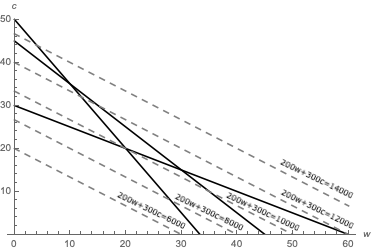
\includegraphics[width=0.35\linewidth]{7-2/3.png}
	\end{figure}
	As we can see, the line of $200 w + 300 c = 10000$ is the max in the feasible region. The intersection means the farmer needs to plant 20 acres of wheat and 20 acres of corn to to maximize the profits.
	
	\item [13a.]
	The largest deviation is $r = \max |y_i - c x_i|$, so the problem is to
	\[
	\text{Min. } r
	\]
	subject to
	\begin{align*}
		r - (11-5c) &\ge 0\\
		r + (11-5c) &\ge 0\\
		r - (25-10c) &\ge 0\\
		r + (25-10c) &\ge 0\\
		r - (54-20c) &\ge 0\\
		r + (54-20c) &\ge 0\\
		r - (90-30c) &\ge 0\\
		r + (90-30c) &\ge 0
	\end{align*}
	Plotting the feasible region (shaded) and the family of lines of the objective function (dashed), we have 
	\begin{figure}[H]
		\centering
		\begin{subfigure}[b]{.4\linewidth}
			\caption{feasible region}
			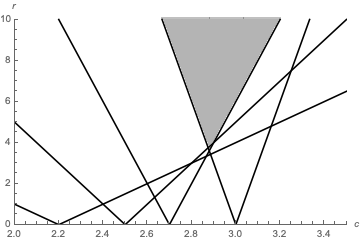
\includegraphics[width=\linewidth]{7-2/13a.png}
		\end{subfigure}
		\hspace{4ex}
		\begin{subfigure}[b]{.4\linewidth}
			\caption{zoom in}
			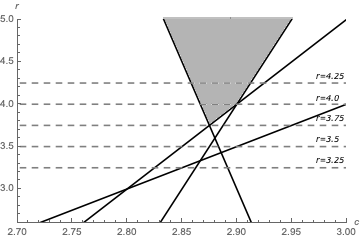
\includegraphics[width=\linewidth]{7-2/13azoom.png}
		\end{subfigure}
	\end{figure}
	As we can see, the line of $r = 3.75$ is the max in the feasible region. The intersection's $c$ coordinate is 2.875. Therefore, $c$ should be 2.875 using Chebyshev's criterion and $y=2.875x$.
	
\end{enumerate}

\section*{Section 7.3}
\begin{enumerate}
	\item [3.]
	According to the figure in problem 3, section 7.2, the objective function at the extreme points is evaluated to be 
	\begin{table}[H]
		\centering
		\begin{tabular}{c*{4}{N}} 
			\toprule
			Extreme point & (0,0) & (0,30) & (20,20) & (33.33,0) \\ \midrule
			$200 w + 300 c$ & 0 & 9000 & 10000 & 6667 \\
			\bottomrule
		\end{tabular}
	\end{table}
	Therefore, to maximize the profits, the farmer need to plant 20 acres of wheat and 20 acres of corn.
	
	\item [7a.]
	According to the figure in problem 13a, section 7.2, at the extreme points $(2.875, 3.75)$ and $(2.9, 4)$, the objective function $r$ equals 3.75 and 4 respectively. Therefore, $c$ should be 2.875 using Chebyshev's criterion and $y=2.875x$.
\end{enumerate}

\end{document}

